\chapter{Machine learning: an overview}
\label{chp:ml}
This chapter is dedicated to the theoretical exploration of some of the most important concepts in
machine learning alongside the various models that have been used in the project. We will begin with
a concise explanation of the more basic concepts linked to machine learning, then we will move to a
theoretical overview of the supervised models of our choice, followed by a brief introduction to
unsupervised machine learning models.

\section{Supervised machine learning}
\label{sec:sml}
Due to the popularization of artificial intelligence in recent times, it's very important to
establish the field to avoid the risk of incurring in misunderstandings. \emph{Machine learning} is
a subset of artificial intelligence, and is a technique that allows us to solve a problem without
the need to actually \emph{invent} an algorithm to solve it (caveat the constraint of having a large
enough dataset to work with). There are many different problems that either lack an algorithmic
solution, or have an inefficient one. In such cases, machine learning is an alternative worth
exploring. The tradeoff of using machine learning instead of 'classic' problem-solving techniques is
that the solution is built using heuristic methods, therefore is not \emph{correct} for the problem~\cite{Rebala2019}.

A supervised machine learning model $\model$ is capable of learning a mapping between an
input space $\ins$ and an output space $\outs$ and then apply this mapping to unseen
data to predict the output~\cite{Cunningham2008}.

Given a problem $\problem$, a specific instance, $\problem_i$, is characterized by a pair
$(\vec{x}_i, y_i)$ where $\vec{x}_i \in \ins$ are vectors taken from an input space $\ins$, usually
highly dimensional, and $y_i \in \outs$ are the expected solutions, which can be expressed using a scalar or vector\footnote{Outcomes will be considered scalars for the rest of this thesis unless explicitly stated}. The single components of every input vector, $\vec{x}_i$, are called \emph{features}, and are values representing a particular aspect of the domain.

A \emph{dataset} is a set containing $n$ problem instances $\dset$. A supervised machine learning model $\model$, trained on $D$, can be used to predict the outcome, $\hat{y}$, of any instance of the problem $\problem_i$. Note that a machine learning model is the result of a statistical process, therefore is susceptible to change unless randomness is kept under control. We will cover this concept in \Cref{chp:problem}

To clarify the concepts just introduced, let us consider the following mock-problem: 'Is it going to rain
tomorrow?'. The dataset $D$ contains $365$ instances of the problem, one per day, for a year. The
input vector for every instance is a set of atmospheric measurements (e.g., temperature, atmospheric
pressure, exposure, humidity, \ldots), each measurement a different feature of the dataset. The
output of every instance $\problem_i$ is a flag answering the question 'did it rain on day $i$?'
with a $1$, for True, and a $0$, for False.

Due to the high grade of complexity of the problem solved in this thesis, future concepts will be clarified
using this exact mock-problem or its variations.

In general, a machine learning problem can be defined as the process of finding the mapping that
relates the input space $\ins$ to the output space $\outs$ by abstracting patterns from
a training set. Conventionally, the output space can be interpreted differently based on
the problem:
\begin{itemize}
	\item $\outs = \{0, 1\}$\footnote{Binary labels can actually vary based on the context, in
		most cases $\{0, 1\}$ can work, but in the literature there are also cases in which
		the output space labels are $\{-1, 1\}$~\cite{ZhouZhi-Hua2021ML}.}, for \emph{binary classification} problems, which are usually associated with pattern recognition tasks, a very easy example of binary classification is our mock-problem. 
	\item $\outs = \{a_1,\ldots, a_m\}$, for \emph{multi-class classification} problems, in
	      which an element can be part of one of the classes in a certain set, a classic
	      example is the character recognition problem, in which a certain character given in
		input can belong to one of 10 different classes (the digits from 0 to 9)~\cite{pal2010handwritten}.
	\item $\outs = \mathbb{R}$, for \emph{regression problems}, which are usually associated
	      with function approximation tasks, an example of regression problem
	      is: 'Based on the current amount of wins for Oklahoma City Thunder\footnote{An
		      amazing \textsc{nba} team}, predict the team's win rate at the end of the season'.
\end{itemize}

Most machine learning models have to go through the same steps, described here below.
\begin{itemize}
	\item \emph{Model selection}: if we consider an instance of a decision tree (introduced in
	      \Cref{sec:dt}), the model can be described through a set of characteristics (e.g.,
	      number of nodes, depth, splitting method, \ldots), all of these are known as
	      \emph{hyperparameters}. An important step of solving a machine learning problem is
	      doing a partial exploration of the hyperparameter space to find the best combination
		for the problem. The search is only partial due to the exponential complexity of the task.
	\item \emph{Model training}: during the training procedure, the instance of the model abstracts
	      patterns from a sample of the dataset, which we will call \emph{training set} $T$.
	\item \emph{Model testing}: during the testing procedure the model performance is tested on
		a part of the dataset, which we will call \emph{test set} or \emph{generalization
		set} $G$. This set is used to understand whether the performance found for $\model$
		is a statistical anomaly (therefore depending on the choice of $T$) or extends also to unseen data.
\end{itemize}

There are many different approaches to splitting a dataset $D$ into a series of separate subsets
for the various tasks involved in the machine learning problem resolution (e.g., model training,
model testing, model selection, \ldots). In the following we will describe two non-trivial aspects of
the basic procedure to split a dataset $D$ into a training set $T$ and a generalization set $G$; a
more complex splitting procedure will be introduced in \Cref{sec:cv}.

\smallskip

Making sure that the distribution of training and test datasets, respectively $T$ and $G$, follow the
same distribution as the original dataset is the first non-trivial aspect of the splitting
procedure. To understand why, let's think about a dataset $\dset$ in which every $\mathbf{x}_i \in
\ins$ is a vector of features describing a patient's conditions (e.g., age, sex, body temperature,
blood saturation, \ldots) and every $y_i \in \outs$ is a string indicating which illness was
diagnosed (e.g., flu, pneumonia, \textsc{covid}, ...). Suppose we want to find a model $\model$ capable of doing a diagnosis effectively: we need to make sure that the least represented illnesses (which are usually the more dangerous ones) are well represented in both $T$ and $G$. If this splitting process was not done correctly we might end up with a model $\model$ that can reliably recognize a common flu but can't correctly identify serious illnesses like pneumonia.

The second non-trivial aspect of the splitting procedure is that it's always necessary to make sure
that the splitting operation is carried out independently for each dataset. Data in the training set
cannot be in the testing set and vice versa. Having such a situation would mean that there is a data
leak from $T$ to $G$, leading to more optimistic performance reads, relaying unjustifed confidence in the model performance.

\smallskip

Data leaks can be a cause of the \emph{overfitting} phenomenon\footnote{
	Data leakage is not the only cause, a model can overfit for many other reasons, such as: the
	training set is too small, the model is too complex and picks up noise, the dataset was not
	cleaned prior to use, \ldots
	}.
Given the generic machine learning problem $\problem$ and a dataset $\dset$, the model $\model$ that solves $\problem$, is said to be overfitting when the training performance is acceptable, but the testing performance is unacceptably bad. This means that the mapping found by $\model$ to link $\ins$ and $\outs$ is too closely related to the specific data chosen to do the training, therefore unable to generalize effectively. In other words, $\model$ is overfitting whenever, instead of abstracting some general patterns from the data, it actually learns peculiarities of the specific training dataset $T$~\cite{ZhouZhi-Hua2021ML}, which are not found later in the testing dataset $G$.

\smallskip

An 'orthogonal' problem to overfitting is the issue of \emph{underfitting}, which is usually caused
by a model not being powerful enough to abstract information from a certain dataset. Whenever a
machine learning model is underfitted for a problem $\problem$, the performance metrics obtained
during training and testing are unacceptably bad, independently of the train and test set
utilized.

\medskip

Since the data at our disposal has already been labelled in previous works~\cite{mariotto2022,
mariotto2022-generic}, we mostly relied on supervised machine learning models, while also leveraging
some unsupervised models for specific approaches. In the following we will be discussing, on a theoretical level, the various supervised models deployed to solve the problem.

\section{Decision Trees}
\label{sec:dt}
This section is a theoretical introduction to decision trees, the implementation we used for the
model is the \emph{DecisionTreeClassifier} class contained in scikit-learn.

\smallskip

A decision tree is a machine learning model based on a tree structure, an example of such a
structure can be seen in \Cref{fig:simple-dt}. Each internal node contains a condition that needs to
be evaluated on one or more features (e.g.,  the root of \Cref{fig:simple-dt} requires us to check
whether the humidity feature of the input is $\geq 80\%$), if the result of the evaluation is true
the computation proceeds with the left child, otherwise the right path will be taken. Once a leaf is
reached, the class associated to the point is identified as the prediction made by the model. If we consider again \Cref{fig:simple-dt} we could say that if the humidity feature for the input is $\geq 80\%$ and the temperature feature is $\geq 10\C$ then it will be classified as 'rain'. Any path leading from root to leaf is known as a \emph{decision path}. It's evident that such structures have a very high degree of explainability and that is why usually they are the first model chosen to solve a machine learning problem.

\medskip

Two are the theoretical concepts we wish to cover in this section: indices and node split
computation, avoiding overfitting through pre- and post- pruning.
\begin{figure}
	\centering
	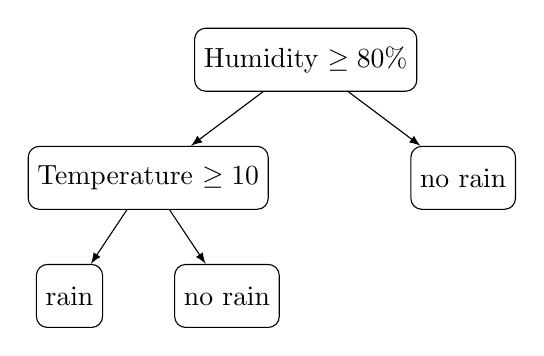
\begin{tikzpicture}[
			% Define styles for nodes
			level 1/.style={sibling distance=40mm},
			level 2/.style={sibling distance=20mm},
			level 3/.style={sibling distance=10mm},
			every node/.style={draw, rectangle, rounded corners, align=center, minimum size=8mm},
			edge from parent/.style={draw, -latex}
		]

		% Root node
		\node {Humidity $\geq 80\%$}
		% First level
		child {node {Temperature $\geq 10\C$}
				% Second level
				child {node {rain}}
				child {node {no rain}}
			}
		child {node {no rain}};
	\end{tikzpicture}
	\caption{A very simple example of decision tree built on the mock problem}
	\label{fig:simple-dt}
\end{figure}
\subsection{Indices and node split computation}
In \Cref{fig:simple-dt} a simple structure for a decision tree was shown, an excellent question in
its regard could be: 'Why this structure and not another one?'. Other than it being a simple
example, nothing is really preventing us from describing the 'rain' event based on different threshold values or different feature sets altogether.
\begin{figure}
	\centering
	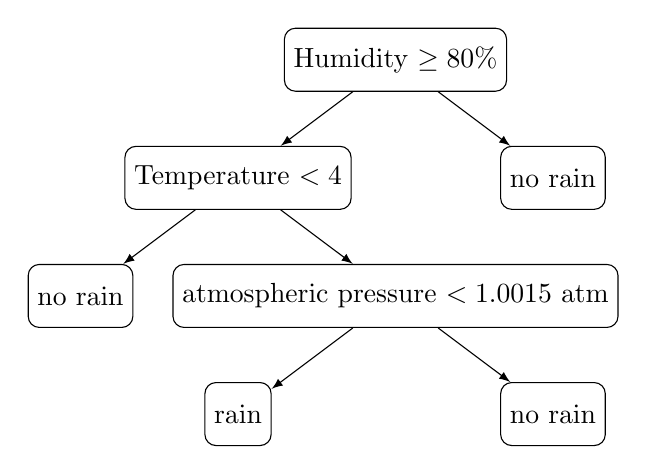
\begin{tikzpicture}[
			% Define styles for nodes
			level 1/.style={sibling distance=40mm},
			level 2/.style={sibling distance=40mm},
			level 3/.style={sibling distance=40mm},
			every node/.style={draw, rectangle, rounded corners, align=center, minimum size=8mm},
			edge from parent/.style={draw, -latex}
		]

		% Root node
		\node {Humidity $\geq 80\%$}
		% First level
		child {node {Temperature $< 4\C$}
				% Second level
				child {node {no rain}}
				child {node {atmospheric pressure $< 1.0015$ atm}
						child{node {rain}}
						child{node {no rain}}
					}
			}
		child {node {no rain}};
	\end{tikzpicture}
	\caption{Another decision tree built on the mock-problem and alternative to
		\Cref{fig:simple-dt}}
	\label{fig:simple-dt-alt}
\end{figure}
The mock tree shown in \Cref{fig:simple-dt-alt} is a different tree compared to the one shown in
\Cref{fig:simple-dt}; and yet they solve the same problem by characterizing it differently.
\Cref{algo:decision-tree} shows how the decision tree is built, the procedure is greedy, since it
tries to pick the best splitting feature with every iteration (at line $10$ the choice is taken
based on a \emph{purity} index applied to the tree nodes, we will clarify the concept later), therefore the resulting trees could be different even if the dataset stays the same.

This variability is due to the stochastic nature of the construction process, as we will see in
\Cref{chp:problem}, there are many things to keep in mind, as well as precautions that can be taken
to make sure that the results do not change with every run.

\begin{algorithm}
	\caption{The decision tree base algorithm taken from
		\cite{ZhouZhi-Hua2021ML}}\label{algo:decision-tree}
	\begin{algorithmic}[1]
		\Require Training set $\dset$ and Feature set $A = \{a_1, \ldots,
			a_d\}$.
		\Ensure A decision tree
		\Function{TreeGenerate}{$D$, $A$}
		\State Generate node $i$;
		\If{All samples in $D$ belong to the same class $C$}
		\State Mark node $i$ as a class $C$ leaf node; \textbf{return node $i$}
		\EndIf
		\If{$A = \emptyset$ \textsc{or} all samples in $D$ take the same
			value on $A$}
		\State Mark node $i$ as a leaf node, its class label is
		the majority in $D$;
		\State \textbf{return node $i$}
		\EndIf
		\State Select the optimal splitting feature $a_*$ from $A$;
		\For{each value $a_*^v$ on $a_*$}
		\State Generate a branch for node $i$;
		\State Let $D_v$ be the subset of samples taking value $a_*^v$ on $a_*$;
		\If{$D_v$ is empty}
		\State Mark this child node as a leaf node;
		\State label t with the majority class of $D$;
		\textbf{return node $i$}
		\Else
		\State use \textproc{TreeGenerate}$(D_v, A \setminus \{a_*\})$ as the child node.
		\EndIf
		\EndFor
		\EndFunction
	\end{algorithmic}
\end{algorithm}

The purity of a node defines how heterogeneous are the samples associated to it. Intuitively, in the
context of our mock-problem: if the distribution of samples arriving to a node $i$ is $15$ labelled
$1$, and $1$ labelled $0$, then the purity of the node is going to be very high.

A split is going to be performed on feature $a$ only if the resulting purity increase is the best
possible. There are many different indices used to compute purity, in the following I will be
covering only those relevant to the parameter grid used in the context of Nested Cross Validation
(described in \Cref{sec:cv}): \emph{Entropy} and \emph{Gini index}.

\subsubsection{Entropy}
We will define \emph{entropy} following the approach in~\cite{gray2011entropy}. Let us consider a
triple $(\Omega, \mathcal{B})$, the first is called \emph{sample space}, the second is a $\sigma$-algebra, which is a collection of elements of $\Omega$ having the following properties:
\begin{itemize}
	\item $\Omega \in \mathcal{B}$;
	\item if $F \in \mathcal{B}$, then $F^C = \{\omega: \omega \notin F\} \in \mathcal{B}$;
	\item if $F_i \in \mathcal{B}, i = 1, 2, \ldots;$ then $\bigcup_i{F_i} \in \mathcal{B}$.
\end{itemize}
We can define the probability space $(\Omega, \mathcal{B}, P)$ and if we consider a discrete random
variable $f$, then we can compute entropy as follows: \[H(f) = - \sum_{a \in A}\].



There are many different ways of defining information entropy, but a more general definition, compared
to the one found in~\cite{ZhouZhi-Hua2021ML}, is found in. Let's consider a
random variable $f$ built on the alphabet $B = \{b_1, \ldots, b_{|B|}\}$ we can define the
partition $\mathcal{Q} = \{Q_i: i = 1, \ldots, |B|\}$ where $Q_i = \{\omega: f(\omega) = b_i\} =
f^{-1}(b_i)$ therefore $\mathcal{Q}$ is a partition of the bigger probability space $\Omega$. Every
partition is chosen based on the outcome of the measurement of the random variable $f$. In the case
of a discrete random variable we can define the information entropy as follows
\begin{equation}
	\label{eq:information-entropy}
	H_p(\mathcal{Q}) = - \sum_{i = 1}^{|B|}{P(Q_i)\log{P(Q_i)}} \enspace;
\end{equation}
this definition of entropy can be easily extended to the dataset case since:
\begin{itemize}
	\item the partition set $\mathcal{Q}$ can be mapped to the dataset $D$,
	\item every partition $Q_i$ can be mapped to the single class of the machine learning
	      problem that is being considered,
	\item the alphabet $B$ can be mapped to the set of possible outcomes of the machine learning
	      problem.
\end{itemize}
Therefore, we can rewrite \Cref{eq:information-entropy} as:
\begin{equation}
	H_p(D) = - \sum_{k = 1}^{|\outs|}p_k \log{p_k} \enspace,
\end{equation}
where $p_k$ denotes the proportion of the $k$-th class inside dataset $D$.

\smallskip

In the case of features with a discrete number of values, the impurity decrease (which is equivalent
to the purity increase) is computed on all possible values for the feature we are splitting on. If we consider our mock-problem, a split could be computed on a feature called 'amount of clouds' which can have one of two values $\{\text{overcast}, \text{clear}\}$. The new node could be built in two different ways and the class distribution for each is different, having different levels of purity based on how well the data is partitioned between the classes 'rain' and 'no rain'.

\smallskip

To choose which of the two nodes to take in our mock-problem using the entropy measure we need to
introduce the concept of \emph{information gain}, which is expressed as follows:
\begin{equation}
	\label{eq:information-gain}
	\textsc{Gain}(D, a) = H_p(D) - \sum_{v = 1}^V\frac{|D^v|}{|D|}H_p(D^v) \enspace.
\end{equation}
The concept expressed by information gain in is that the amount of information gained by doing a split of dataset $D$ on feature $a$ is given by the entropy of dataset $D$ at the moment of the split from which we remove the entropy of the dataset resulting from the split of feature $a$ at every value $v$ scaled by the ratio between the cardinality of the new dataset to the cardinality of the original dataset.

\smallskip

The feature used to perform the split on is going to be the one with the highest possible
information gain. It's very important to notice that information gain is an index biased towards
features that have many different values (and therefore $|D^v|$ is small). In the case of our mock
problem, if we consider 'status of the sky' and we compare it to another feature containing many
different splitting values, for example 'cloud color', which might assume the following values
$\{\text{white}, \text{light grey}, \text{grey}, \text{black}, \text{pink}, \text{orange},
	\text{red}\}$, it's clear that the $|D^v|/|D|$ is going to be lower for each of them, therefore
leading to a lower entropy decrease and a higher information gain.

\emph{Gain ratio} is an alternative to information gain, it is defined as follows
\begin{equation}
	\label{eq:gain-ratio}
	\textsc{GainRatio}(D, a) = \frac{\textsc{Gain}(D, a)}{\textsc{iv}(a)}
\end{equation}
the \textsc{iv} function is the \emph{intrinsic value} of feature $a$
\begin{equation}
	\label{eq:intrinsic-value}
	\textsc{iv}(a) = - \sum_{v = 1}^V\frac{|D^v|}{|D|} \log{\frac{|D^v|}{|D|}} \enspace.
\end{equation}
Due to how intrinsic value is defined, the gain ratio corrects the bias of the information gain
towards features with a higher number of values, but it also makes it biased towards features with a lower amount of values~\cite{ZhouZhi-Hua2021ML}.

\smallskip

The actual implementation of the decision tree model in the scikit-learn library is an optimized version of the \textsc{cart} algorithm, similar to the \textsc{c4.5} algorithm proposed by Quinlan in~\cite{quinlan2014c4}.

\subsubsection{Gini index}
The original \textsc{cart} algorithm conceptualized by Breiman et al. in
1984~\cite{breiman1984classification} used Gini index to compute the best splitting feature for
every node. The Gini value of a dataset can be computed as shown here below
\begin{equation}
	\label{eq:gini-value}
	\textsc{Gini}(D) = \sum_{k = 1}^{|\outs|}\sum_{k' \neq k} p_kp_{k'} = 1 - \sum_{k =
		1}^{|\outs|}p_k^2 \enspace.
\end{equation}
As explained in~\cite{ZhouZhi-Hua2021ML}, Gini value can be interpreted as the
likelihood of taking samples from two different classes by drawing them randomly from the
dataset, the lower the $\textsc{Gini}(D)$, the higher the purity of a node. Gini index can be
computed as the weighted sum of all the Gini values associated to the datasets obtained by doing a
split with respect to a specific value
\begin{equation}
	\label{eq:gini-index}
	\textsc{GiniIdx}(D,a) = \sum_{v = 1}^V\frac{|D^v|}{|D|} \textsc{Gini}(D^v) \enspace.
\end{equation}

The best splitting feature is going to be the one with the smallest Gini index overall.

\subsection{Avoiding overfitting through pre- and post- pruning}
As was argued in the beginning of the section (cfr. \Cref{sec:dt}), decision trees have an extremely simple structure and the results are easy to interpret.

Overfitting is probably the biggest drawback of decision trees, as shown in~\cite{overfitting-dt-erblin}. Since the model tries to partition the space based on the purity of the nodes, it's important to make sure that the splitting rules utilized are not overly specific. Two techniques are commonly explored in the literature to prevent overfitting: \emph{pre-pruning} and \emph{post-pruning}.

\smallskip

Pre-pruning forces an early stop of the algorithm whenever a series of conditions allow it, in other
words, pre-pruning is a group of techniques meant to keep the size of the decision tree in
check~\cite{ZhouZhi-Hua2021ML, bramer2007principles, fisher1996learning}. Even if the split produces a decrease in the impurity of the current node it might be detrimental to proceed greedily, a couple of examples could clarify this suggestion:
\begin{itemize}
	\item It might happen that the node is labelled 'Class B', while containing a handful of
		samples from 'Class A'. If the set of outcasts is small enough doing a split to
		classify them correctly only introduces more complexity in the tree which usually is
		not beneficial to the end result.

	\item If we have a tree that is already deep, adding even more splits to make the nodes purer
		only makes it both more complicated and more likely to overfit the training data.
\end{itemize}

The specific pre-pruning conditions that can be checked in scikit-learn are the following.
\begin{itemize}
	\item The tree \emph{depth}, avoiding a complex tree structure by cutting the depth, which is
	      probably one of the easiest forms of pre-pruning.
	\item The \emph{impurity decrease} stops nodes from splitting when the decrease in impurity
	      of the children is not higher than a certain threshold. If the threshold is too high
	      then the tree will probably underperform, if it's too low then the tree is likely going to
	      overfit.
	\item The \emph{number of elements to split}, which defines how many samples must be
		contained in a node to make it an internal node for the tree.
\end{itemize}

Post-pruning is the alternative to pre-pruning, the essential difference between the two is that
post-pruning is done after the tree has been fully constructed. In the a posteriori phase,
a subset of branches will be chosen to be pruned based on the impurity decrease that they provide.
Scikit-learn is working with Cost Complexity Pruning (\textsc{ccp}), introduced in~\cite{breiman1984classification}.

\section{Ensemble learning}
\label{sec:el}
In the previous chapter we introduced decision trees, and we have talked about their
strengths and weaknesses; providing some instruments to counter their shortcomings. Sometimes,
despite our efforts, the decision tree model is simply not enough for the task at hand. If we don't
want to give up the explainability, in favor of higher performance, we can construct an ensemble.

An ensemble contains a group of weaker learners: grouping produces a series of effects, two of which are
very important (to clarify the concepts we will consider the dynamics of a basketball team during a
game):
\begin{itemize}
	\item Different learners are able to grasp different aspects of the problem, which would be
		either impossible or complicated for single models. If we consider our example, each
		player covers different positions, which do not fit his teammates (this doesn't
		entail that there is no player capable of, if needed, covering more than one
		position; which is usually a characteristic of the best players in the team).
	\item Using a group of models alleviates the shortcomings of the weaker learners. If we consider our example: the weaker players, and lesser role players, stay on the bench while the main rotation is playing; but can still contribute with some quality minutes when the main rotation is facing a difficulty.
\end{itemize}

In~\cite{ZhouZhi-Hua2021ML} a proof was given to relate the error rate of an ensemble with its size,
which we outline here below.

Let us consider an ensemble of size $T$, we will refer to the $i$-th learner in the ensemble as
$h_i$. Let us call the ground truth function $f$ and let the probability of learner $h_i$
misclassifying $\vec{x} \in \ins$ be
\begin{equation}
	\label{eq:error-rate}
	Pr(h_i(\vec{x}) \neq f(\vec{x})) = \epsilon \enspace.
\end{equation}
Assuming that the ensemble is solving a binary classification problem, then the class labels can be defined as $y \in \{-1, +1\}$. The ensemble will aggregate the predictions by using a simple majority algorithm; 
\begin{equation}
	\label{eq:ensemble-aggregation}
	F(\vec{x}) = \sign\left(\sum_{i = 1}^{T}h_i(\vec{x})\right) \enspace.
\end{equation}
Since the probability of a base learner of being correct is $1 - \epsilon$, then the ensemble
correctly classifies a sample only if more than half of the learners correctly identify the sample.
If we assume the learners to be independent of each other, then we can model the probability of the
ensemble being correct using a Binomial distribution, $Bin(k, 1 - \epsilon)$:
\begin{equation}
	\label{eq:succ-probability}
	\begin{aligned}
		Pr(\text{success}) & = Pr\left(\text{at least } \left\lceil{\frac{T}{2}}\right\rceil \text{ correctly identify
		the sample}\right)
		\\
			   & = \sum_{k = \lceil{T / 2}\rceil}^T \binom{T}{k} (1 - \epsilon)^k
			   \epsilon^{T - k} \enspace.
	\end{aligned}
\end{equation}
Since we are interested in finding a bound for the ensemble error rate, we are interested in the
complement of $Pr(\text{success})$, which is $Pr(\text{insuccess}) = Pr(F(\vec{x}) \neq
f(\vec{x}))$. The ensemble misclassifies a sample only if the number of learners that can correctly
classify the model is less than half, therefore $Pr(\text{insuccess})$ can be defined as
\begin{equation}
	\label{eq:insucc-probability}
	Pr(\text{insuccess}) = Pr(F(\vec{x}) \neq f(\vec{x})) = \sum_{k = 0}^{\lfloor{T / 2}\rfloor}
	\binom{T}{k} (1 - \epsilon)^k \epsilon^{T - k} \enspace.
\end{equation}
Finally, we can exploit Hoeffding's inequality~\cite{ZhouZhi-Hua2021ML}
on~\ref{eq:insucc-probability}, obtaining an upper bound for the error rate of the ensemble.
\begin{equation}
	\label{eq:hoeffding}
	\sum_{k = 0}^{\lfloor T / 2 \rfloor}\binom{T}{k} (1 - \epsilon)^k\epsilon^{T - k} \leq
	\exp\left(-\frac{1}{2}T(1 - 2\epsilon)^2\right) \enspace.
\end{equation}
The result is telling us that the error rate of the ensemble falls exponentially with the
number of base learners $T$. This proof is based on the non-trivial assumption that the base
learners are independent of each other, which is something that doesn't apply in the practical
case, since the models are trained on the same dataset for the same problem $\problem$.

In the next two sections we will introduce bagging and random forests, which are two very similar
ensemble algorithms.

\subsubsection{Bagging}

Bagging, introduced by Leo Breiman~\cite{Breiman1996}, is a method for generating multiple
versions of a base predictor that are then aggregated in a single model, as outlined in
\Cref{algo:bagging} following~\cite{ZhouZhi-Hua2021ML, Bauer1999}.
\begin{algorithm}
	\caption{The bagging algorithm, taken from~\cite{Bauer1999}}\label{algo:bagging}
	\begin{algorithmic}[1]
		\Require A training dataset $\dset$, a base learner $\mathcal{L}$, a certain number
		of training rounds $T$.
		\Ensure An ensemble model capable of aggregating predictions.
		\Function{Bagging}{$D$, $\mathcal{L}$, $T$}
		\For {$t = 1, \ldots, T$}
		\State $D_{bs}$ obtained by bootstrap sampling from $D$
		\State $h_t = \mathcal{L}(D_{bs})$ 
		\EndFor
		\State \textbf{return} $H(\vec{x}) = \argmin_{y \in \outs}\sum_{t : h_t(\vec{x}) =
		1} 1$
		\EndFunction
	\end{algorithmic}
\end{algorithm}

\Cref{algo:bagging} can be described as follows: given a dataset $\dset$ of size $n$, we create a new
dataset of size $n$ ($D_{bs}$ in \Cref{algo:bagging}) by randomly sampling with replacement from
$D$~\footnote{The technique is known as bootstrap sampling~\cite{ZhouZhi-Hua2021ML}}. If we repeat
the procedure $T$ times we obtain $T$ different datasets of size $n$, which can be used to train
different base learners. Once the training is over, predictions can be done on inputs and the
results can be aggregated using different techniques (e.g., majority voting or averaging).

Since $D_{bs}$ is being built sampling from $D$ with replacement it's interesting to give an
estimate of the number of samples that are not being used to build the $i$-th dataset. Since the
probability of being picked is $1 / n$, and doesn't change with the iteration, then the probability of not being picked is $1 - 1 / n$.

Considering the extreme case, $n \rightarrow \infty$, and then computing the probability of a sample
not being picked for $n$ different draws. \begin{equation}
	\label{eq:bagging-limit}
	\lim_{n \rightarrow \infty} \left(1 - \frac{1}{n}\right) = \frac{1}{e} \approx 0.368
	\enspace,
\end{equation}
We expect the $36.8\%$ of the data in $D$ to remain unused every time a new dataset $D_{bs}$ is
being built by bootstrapping. Since this data would be 'lost', we can implement different mechanisms
to take advantage of the surplus; an example could be a variation of the train-test split seen in the beginning of the chapter: if we keep track of the data used for $D_{bs}$, what remains can be put in $V_{bs}$, which is called validation set, and can be used to understand how much the single learner is able to generalize after training.

\subsubsection{Random Forests}

Random forests are an extension of the Bagging model described above, conceived by Leo Breiman~\cite{Breiman2001}. While decision trees perform the splitting procedure for every node by selecting the feature that yields the best impurity reduction, random forests pick the feature that yields the best impurity decrease from a random subset of features of size $k$. The value of $k$ controls how random the splitting procedure is going to be, if $k = d$, where $d$ is the size of the feature set, then the behavior of the random forest is the same as the decision tree introduced in the last section, if $k = 1$, then the splitting feature is chosen randomly.

Despite the relative simplicity of the model, random forests provide a high level of performance,
accompanied by the classic explainability of decision trees (with the added complexity of
having an ensemble of classifiers).

\section{SVM}
\label{sec:svm}
With this section, we leave behind the tree-based models to talk about our benchmark. An
\svm\ is a model characterized by very high performance but low explainability: in this
section we will understand its the theoretical foundations~\cite{ZhouZhi-Hua2021ML}.

\smallskip

Let us consider a binary classification problem on dataset $\dset$ with labels $y \in \{-1, +1\}$.
Handling the classification task means finding a hyperplane that is able to divide the points in the
dataset 'reasonably well'. Since the number of such hyperplanes is infinite there are two
essential observations to be made:
\begin{enumerate}
	\item the space of the solutions cannot be checked thoroughly, therefore we will never know
	      if the chosen hyperplane is the best, or if there is another one that yields better
	      performance;
	\item the chosen hyperplane will be fitted on the dataset used for training, but we can
		ensure good generalization performance by choosing the hyperplane that maximizes the
		\emph{margin}, which is the minimal distance between the decision surface and the
		'hardest' points in the dataset.
\end{enumerate}
The 'hardest' points are the ones closest to the hyperplane, referred to as \emph{support vectors}.

\smallskip

We can express any hyperplane in space as a function of a normal vector $\vec{w}$ controlling the direction of the hyperplane and a bias value $b$ controlling the distance of the hyperplane from the origin:
\begin{equation}
	\label{eq:hyperplane}
	\vec{w}^\top\vec{x} + b = 0 \enspace.
\end{equation}
For any given point in space we can compute its distance from the hyperplane
\begin{equation}
	\label{eq:hyperdistance}
	r = \frac{|\vec{w}^\top\vec{x} + b|}{||\vec{w}||} \enspace.
\end{equation}
If the hyperplane can perfectly divide the points in the two classes, we have
\begin{equation}
	\label{eq:system}
	\begin{cases}
		 & \vec{w}^\top\vec{x}_i + b > 0, \hspace{10pt} y_i = +1 \enspace, \\
		 & \vec{w}^\top\vec{x}_i + b < 0, \hspace{10pt} y_i = -1 \enspace.
	\end{cases}
\end{equation}
We can give a stronger condition, which only works for the support vectors, and is based on the
distance defined in~\ref{eq:hyperdistance}:
\begin{equation}
	\label{eq:svm-system}
	\begin{cases}
		 & \vec{w}^\top\vec{x}_i + b \geq +1, \hspace{10pt} y_i = +1 \enspace, \\
		 & \vec{w}^\top\vec{x}_i + b \leq -1, \hspace{10pt} y_i = -1 \enspace.
	\end{cases}
\end{equation}
The margin, defined here below, is the total distance between two support vectors belonging to different classes:
\begin{equation}
	\label{eq:margin}
	\gamma = \frac{2}{||\vec{w}||} \enspace.
\end{equation}

As was said in the beginning of this section, we want to find the best separating hyperplane,
ensuring the best generalization performance, therefore it has to be at a reasonable distance from
the hardest points in the training set. We can express this problem via a maximization problem: we
want to maximize the margin in~\ref{eq:margin}, subject to the constraints of
equation~\ref{eq:svm-system}. Maximizing the margin means maximizing $||\vec{w}||^{-1}$ which is
equivalent to minimizing $||\vec{w}||^2$, taken for simplicity. The result is the primal form of
\svm:
\begin{equation}
	\label{eq:primal}
	\begin{aligned}
		\max_{\vec{w}, b}        & \frac{1}{2}||\vec{w}||^2                                            \\
		\text{s.t.}\hspace{10pt} & y_i(\vec{w}^\top\vec{x}_i + b) \geq 1 \hspace{10pt}i = 1,
		\ldots, n \enspace.
	\end{aligned}
\end{equation}
This is a quadratic programming problem, and there are libraries providing solvers for it, but there
are other methods that allow us to compute a solution with a higher grade of efficiency. We can
introduce \emph{Lagrange multipliers} $\alpha_i$ and the Lagrangian function.
\begin{equation}
	\label{eq:lagrangian}
	\lag(\vec{w}, b, \vec{\alpha}) = \frac{1}{2} ||\vec{w}||^2 + \sum_{i = 1}^{n}{\alpha_i (1 -
	y_i(\vec{w}^\top\vec{x}_i + b))} \enspace.
\end{equation}
If we compute the partial derivatives of the Lagrangian with respect to $\vec{w}$ and $b$ we obtain:
\begin{equation}
	\label{eq:pd-lagrangian}
	\begin{aligned}
		 & \frac{\partial{\lag}}{\partial{\vec{w}}} = \vec{w} - \sum_{i = 1}^n
		\alpha_iy_i\vec{x}_i \enspace,                                                  \\
		 & \frac{\partial{\lag}}{\partial{b}} = \sum_{i = 1}^n \alpha_iy_i \enspace.
	\end{aligned}
\end{equation}
By setting the partial derivatives to zero, and substituting the first in~\ref{eq:lagrangian}, we
can get rid of the normal vector dependency and the \emph{dual} problem can be defined as a function
of the sole $\vec{\alpha}$. The dual problem is
\begin{equation}
	\label{eq:dual}
	\begin{aligned}
		\max_{\vec{\alpha}}       & \left(\sum_{i = 1}^n{\alpha_i} - \frac{1}{2}\sum_{i =
		1}^n\sum_{j = 1}^n{\alpha_i\alpha_j y_i y_j \vec{x}_i^\top\vec{x}_j}\right)               \\
		\text{s.t.} \hspace{10pt} & \sum_{i = 1}^n{\alpha_i y_i} = 0 \hspace{10pt}
		\alpha_i \geq 0 \hspace{3pt} \forall i \enspace.
	\end{aligned}
\end{equation}
The hyperplane can be modelled as follows, in virtue of the substitution found for $\vec{w}$
in~\ref{eq:pd-lagrangian}:
\begin{equation}
	\label{eq:of}
	f(\vec{x}) = \vec{w}^\top\vec{x} + b = \sum_{i = 1}^n\alpha_iy_i\vec{x}_i\vec{x} + b
\end{equation}
Since~\ref{eq:primal} is an optimization problem with inequality constraints, it must satisfy
Karush-Kuhn-Tucker necessary conditions~\cite{kkt1951}\footnote{For a small ex-cursus on
\textsc{kkt} conditions, refer to \Cref{app:kkt}.}. Solving the primal is equivalent to solving the
dual subject to the following constraints:
\begin{equation}
	\label{eq:kkt-constraints}
	\begin{cases}
		 & \alpha_i \geq 0 \enspace,                   \\
		 & y_if(\vec{x}_i) - 1 \geq 0 \enspace,        \\
		 & \alpha_i(y_if(\vec{x}_i) - 1) = 0 \enspace.
	\end{cases}
\end{equation}
Constraints in \Cref{eq:kkt-constraints} reveal that, for every point in the training set $(\vec{x}_i, y_i)$, only two scenarios are possible:
\begin{enumerate}
	\item if $\alpha_i = 0$, then the point $(\vec{x}_i, y_i)$ is not influencing~\ref{eq:of}.
	\item If $\alpha_i > 0$ then the third constraint in~\ref{eq:kkt-constraints} yields
		$y_if(\vec{x}_i) = 1$ meaning that the point is laying on the maximum margin hyperplanes, therefore it's a support vector.
\end{enumerate}
Which leads us to a very important conclusion: once the training is completed, the model can be entirely
described by using only support vectors, since they are the ones that yield a contribution in the
calculation of~\ref{eq:of}.

There are different techniques to solve the dual problem~\ref{eq:dual}: quadratic programming
solvers or Sequential Minimal Optimization \textsc{smo} method.

Proposed in \cite{platt1998} it consists of an iterative resolution of the problem, by successive
identifications of local approximations of $\alpha_i$, while keeping all other parameters frozen as
constants. Platt's algorithm, compared to the competition (Osuna's~\cite{osuna1997} and Chunking),
spends less time doing Lagrange multiplier optimization during training. In the project we used
Support Vector Classifiers (\svcs) and their implementation in scikit-learn relies upon
\textsc{libsvm}, which is an open source library to work with \svms. The library was born in $2000$,
initially written in C++ is now used by most modern languages and, to decompose the dual problem,
uses a variant of the \textsc{smo} method~\cite{fang2005}.

\subsection{Soft-margin SVM}
\label{sec:se-svm}
The method explained until now provides a solution to the primal problem~\ref{eq:primal}, which is meant to
have perfect accuracy, meaning that no classification errors are accepted. This is a solution that
is neither advisable nor possible in most cases, due to the problem of linear separability, which we
will address in \Cref{sec:kernel-functions}.

For this reason the \emph{soft margin} \textsc{svm} model was defined: its formulation of the solution
allows a relaxation of the constraints, therefore, a certain number of classification errors.
Since the number of errors needs to be minimized, we can rewrite the objective of equation~\ref{eq:primal} as
\begin{equation}
	\label{eq:sm-primal}
	\min_{\vec{w}, b} \frac{1}{2}||\vec{w}||^2 + C\sum_{i = 1}^n \ell_{0 / 1}(y_i (\vec{w}^\top
	\vec{x}_i + b) - 1) \enspace,
\end{equation}
where $C > 0$ is a regularization constant and $\ell_{0 / 1}$ is the $0/1$ loss. Solving directly the equation can be complicated, due to the poor mathematical properties of the $0/1$ loss function, even if there are approximate methods to minimize it~\cite{nguyen2013}, usually a convex loss function is used to replace it.

Soft margin \textsc{svm} is defined by substituting $0/1$ loss with hinge loss, a convex function for binary classifiers defined as $\ell(y) = \max(0, 1 - ty)$ where $y$ is the raw output of the classifier and $t$ is the label associated to the output, and then adding slack variables $\xi_i \geq 0$. The primal problem can be easily rewritten as
\begin{equation}
	\label{eq:sm-primal-final}
	\begin{aligned}
		\min_{\vec{w}, b}         & \frac{1}{2}||\vec{w}||^2 + C\sum_{i = 1}^n \xi_i
		\enspace,\\
		\text{s.t.} \hspace{10pt} & y_i(\vec{w}^\top\vec{x}_i + b) \geq 1 - \xi_i \enspace,    \\
		                          & \xi_i \geq 0 \hspace{10pt}i = 1, \ldots, n \enspace.
	\end{aligned}
\end{equation}
If we apply the Lagrange multipliers method the Lagrangian will be dependent on: the slack
variables, normal vector $\vec{w}$, the Lagrange multipliers $\vec{\alpha}, \vec{\mu}$ and the bias $b$. Tre function can be expressed as
\begin{equation}
	\label{eq:sm-lagrangian}
	\begin{aligned}
		\mathcal{L}(\vec{w}, b, \vec{\alpha}, \vec{\xi}, \vec{\mu}) & =
		\frac{1}{2}||\vec{w}||^2 + C\sum_{i = 1}^n \xi_i                                                                                                               \\
		& + \sum_{i = 1}^n \alpha_i(1 - \xi_i - y_i(\vec{w}^\top\vec{x}_i + b))
		  + \sum_{i = 1}^n\mu_i\xi_i \enspace.
	\end{aligned}
\end{equation}
By setting the partial derivatives to $0$, just as was done for the generic \textsc{svm}, and doing
some substitutions we obtain the final form of the dual problem for the soft margin \textsc{svm};
\begin{equation}
	\label{eq:sm-dual-final}
	\begin{aligned}
		\max_{\vec{\alpha}}       & \sum_{i = 1}^n \alpha_i - \frac{1}{2}\sum_{i = 1}^n\sum_{j =
		1}^n\alpha_i\alpha_jy_iy_j\vec{x}_i^\top\vec{x}_j \enspace,                                        \\
		\text{s.t.} \hspace{10pt} & \sum_{i = 1}^n\alpha_iy_i = 0 \enspace,                              \\
		                          & 0 \leq \alpha_i \leq C \hspace{10pt} i = 1, \ldots, n
					  \enspace.
	\end{aligned}
\end{equation}
Since the dual problem has a similar structure to equation~\ref{eq:dual}, the same conclusions
apply. We can also extract the \textsc{kkt} conditions, which are:
\begin{equation}
	\label{eq:sm-kkt}
	\begin{cases}
		 & \alpha_i \geq 0, \hspace{10pt}\mu_i \geq 0 \enspace, \\
		 & y_if(\vec{x}_i) - 1 + \xi_i \geq 0 \enspace,         \\
		 & \alpha_i(y_if(\vec{x}_i) - 1 + \xi_i) = 0 \enspace,  \\
		 & \xi_i \geq 0, \hspace{10pt} \mu_i\xi_i = 0 \enspace.
	\end{cases}
\end{equation}
As was done previously, we can draw conclusions by checking the \textsc{kkt} constraints:
\begin{itemize}
	\item If $\alpha_i = 0$, then the sample has no impact on the hyperplane's equation.
	\item When $\alpha_i > 0$, $y_if(\vec{x}_i) = 1 - \xi_i$, therefore the point is a
		support vector.
\end{itemize}

In the following section we will address the linear separability assumption we have implicitly made
until this moment.

\subsection{Kernel funtions}
\label{sec:kernel-functions}
Until now the topic was treated under the important assumption that the points in the dataset are
linearly separable, but it's known that this condition rarely holds in practice. To address the issue the
problem is moved to a higher dimensionality space through a mapping $\phi(\cdot)$, this is done in
the hope that increasing the number of dimensions will make the data linearly separable.
From~\cite{cover1965} we have the guarantee that given a set of $N$ points in Euclidean
$d$-dimensional space, then the number of ways we can split the points in two non-intersecting sets
is
\begin{equation}
	\label{eq:dichotomies}
	C(N, d) = 2 \sum_{k = 0}^{d - 1}\binom{k}{N - 1} \enspace.
\end{equation}

Given a data-point $\vec{x} \in \ins$, we call $\phi(\vec{x})$ its high-dimensionality image.
Then~\ref{eq:hyperplane} can be rewritten as
\begin{equation}
	\label{ep:hd-hyperplane}
	f(\vec{x}) = \vec{w}^\top \phi(\vec{x}) + b \enspace.
\end{equation}
Using equation~\ref{ep:hd-hyperplane} and following the steps used in the beginning of \Cref{sec:svm},
it's possible to redefine both the primal and the dual problems, respectively as
\begin{equation}
	\label{eq:hd-primal}
	\begin{aligned}
		 & \max_{\vec{w}, b}\frac{1}{2}||\vec{w}||^2                                                         \\
		 & \text{s.t.}\hspace{10pt}y_i(\vec{w}^\top\phi(\vec{x}_i) + b) \geq 1 \hspace{10pt}i = 1, \ldots, n
	\end{aligned}
\end{equation}
\begin{equation}
	\label{eq:hd-dual}
	\begin{aligned}
		 & \max_{\vec{\alpha}}\left(\sum_{i = 1}^n{\alpha_i} - \frac{1}{2}\sum_{i =
		1}^n\sum_{j = 1}^n{\alpha_i\alpha_j y_i y_j \phi(\vec{x}_i)^\top\phi(\vec{x}_j})\right) \\
		 & \text{s.t.} \sum_{i = 1}^n{\alpha_i y_i} = 0 \hspace{10pt} i = 1, \ldots, n
		 \hspace{10pt}\alpha_i \geq 0 \hspace{3pt} \forall i \enspace.
	\end{aligned}
\end{equation}

It would now be necessary to compute a solution for the dual problem, which means computing the
internal product $\langle\phi(\vec{x}_i), \phi(\vec{x}_j)\rangle$. Since the problem was moved to a
high dimensional space, it might be computationally expensive operation, especially because the
number of dimensions of the final space is not known a-priori.

%%%%%%%%%%%%%%%%%%%%%%%%%
% THE KERNEL-TRICK DOESN'T PROVIDE AN APPROXIMATION OF THE INNER PRODUCT BUT IT COMPUTES THE ACTUAL
% VALUE. THIS IS THANKS TO THE FACT THAT WE ARE DOING AN EXTENSION TO RKHS SPACE (REPLICATING KERNEL
% HILBERT SPACE)
%%%%%%%%%%%%%%%%%%%%%%%%%
To avoid having to compute such a product, we define a function, known as \emph{kernel} function
$\kappa(\cdot, \cdot)$ which actually defines the inner-product. We can rewrite~\ref{eq:hd-dual} to use the newly introduced function. 
\begin{equation}
	\label{eq:hd-dual-kf}
	\begin{aligned}
		 & \max_{\vec{\alpha}}\left(\sum_{i = 1}^n{\alpha_i} - \frac{1}{2}\sum_{i =
		1}^n\sum_{j = 1}^n{\alpha_i\alpha_j y_i y_j \kappa(\vec{x}_i, \vec{x}_j)}\right) \\
		 & \text{s.t.} \sum_{i = 1}^n{\alpha_i y_i} = 0 \hspace{10pt} i = 1, \ldots, n
		 \hspace{10pt} \alpha_i \geq 0 \hspace{3pt} \forall i
	\end{aligned}
\end{equation}

If we solve the problem using the same procedure applied in the beginning of \Cref{sec:svm}, we obtain
an expression of the hyperplane which is dependent from the kernel function $\kappa$.
\begin{equation}
	\label{eq:hd-of}
	f(\vec{x}) = \sum_{i = 1}^n\alpha_iy_i\kappa(\vec{x}_i, \vec{x}) + b
\end{equation}

Until now we have used the kernel function but without giving a definition for it; that is due to its
dependence from the mapping $\phi$. Such mapping is unknown in most practical cases; however a
theorem~\cite{learning-with-kernels} grants us that if we can find a symmetric function
$\kappa(\cdot, \cdot): \ins \times \ins \rightarrow \ins$, then $\kappa$ is a kernel function if and
only if, however chosen the dataset $D = \{\vec{x}_1, \allowbreak\ldots\allowbreak, \vec{x}_m\}$,
the following kernel matrix $\mathbf{K}$ is positive semidefinite:
\begin{equation}
	\label{eq:kernel-matrix}
	\mathbf{K} =
	\begin{bmatrix}
		\kappa(\vec{x}_1, \vec{x}_1) & \kappa(\vec{x}_1, \vec{x}_2) & \ldots &
		\kappa(\vec{x}_1, \vec{x}_m)                                                  \\
		\kappa(\vec{x}_2, \vec{x}_1) & \kappa(\vec{x}_2, \vec{x}_2) & \ldots &
		\kappa(\vec{x}_2, \vec{x}_m)                                                  \\
		\ldots                       & \ldots                       & \ddots & \ldots \\
		\kappa(\vec{x}_m, \vec{x}_1) & \kappa(\vec{x}_m, \vec{x}_2) & \ldots &
		\kappa(\vec{x}_m, \vec{x}_m)                                                  \\
	\end{bmatrix} \enspace.
\end{equation}
Now that a reliable technique to find kernel functions has been defined, it's important to find the
best kernel function. Since the choice of the kernel determines how the points are mapped in
high-dimensional space, and therefore how good the separating hyperplane is going to be.

\section{Unsupervised models}
\label{sec:uml}
With \svms\ we leave supervised models behind, in this chapter we are going to consider unsupervised
machine learning, capable of extrapolating patterns from unlabelled data.

Unsupervised machine learning models, contrarily to the supervised case, are trained on datasets
that do not contain an expected answer $y_i$ for instance $\problem_i$.

This section is going to be dedicated to explore the theory behind the $k$-means clustering
algorithm: once again the main material used is~\cite{ZhouZhi-Hua2021ML}.

\section{Clustering with k-means}
\label{sec:kmeans}
Given a dataset $\udset$ a clustering algorithm partitions the data into non-intersecting sets
known as \emph{clusters}: the data is grouped based on how similar they are; ideally, the more two
points are similar, the closer they should be.

If, on the one hand, these algorithms are capable of giving us an idea of the
meaning of the points, as well as a hint about the nature of the relations that have with each
other; on the other one, understanding the results of a clustering procedure is not as
straightforward as it sounds. An explanation to the partitioning has to be found by conferring with
experts in the field of interest.

Before introducing the $k$-means algorithm we are going to explore the two most important concepts
in clustering: performance measures and distance calculation.

\subsubsection{Performance measures}
\label{ssec:performance-measures}
Clustering algorithms have their own set of metrics, also known as \emph{validity indices}. Common
scores like \emph{accuracy} and \emph{recall} cannot be used because the dataset doesn't have an
expected class to compare the prediction with~\footnote{
	These and more scores for supervised learning models will be explored in
	chapters~\ref{chp:qrp}--~\ref{chp:qlp}. The metrics used will be introduced in
	chapter~\ref{chp:problem}.
}. In the clustering environment there are indices that allow us to mathematically
express the fact that points belonging to the same cluster are similar (\emph{intra-cluster
similarity}); while points that belong to different clusters have to be different enough (\emph{inter-cluster similarity}).

\smallskip

Over the years many different indices have been defined, all of them using different aspects of the
cluster structure and rating them on a different scale. All of this scoring methods can be divided
in two big families:
\begin{itemize}
	\item \emph{external indices}, which compare the clustering result against a reference model,
	\item \emph{internal indices}, which evaluate clustering performance without using a
		reference model; using a certain set of measures that can be performed on the
		clustering instance itself.
\end{itemize}
We will begin by considering external indices. Suppose that a clustering algorithm $\model$ has
constructed a partition $\mathcal{C} = \{C_1, \ldots, C_k\}$ while a reference model $\model^*$
constructed partition $\mathcal{C}^*=\{C^*_1, \ldots, C^*_h\}$. Each cluster $C_i$ and $C^*_i$ is
labelled with a value $\lambda_i$ and $\lambda^*_i$. Grouping all labels together we obtain vectors
$\vec{\lambda}$ and $\vec{\lambda}^*$. For each pair of samples $(\vec{x}_i, \vec{x}_j)$ we can
define terms: 
\begin{equation}
	\label{eq:clustering-terms}
	\begin{aligned}
		a =|SS|, \hspace{10pt} &SS = \{(\vec{x}_i, \vec{x}_j) | \lambda_i = \lambda_j, \lambda^*_i =
		\lambda^*_j, i < j\} \enspace, \\
		b =|SD|, \hspace{10pt} &SD = \{(\vec{x}_i, \vec{x}_j) | \lambda_i = \lambda_j, \lambda^*_i
		\neq \lambda^*_j, i < j\} \enspace, \\
		c =|DS|, \hspace{10pt} &DS = \{(\vec{x}_i, \vec{x}_j) | \lambda_i \neq \lambda_j, \lambda^*_i =
		\lambda^*_j, i < j\} \enspace, \\
		d =|DD|, \hspace{10pt} &DD = \{(\vec{x}_i, \vec{x}_j) | \lambda_i \neq \lambda_j,
		\lambda^*_i \neq \lambda^*_j, i < j\} \enspace.
	\end{aligned}
\end{equation}
The $i < j$ constraint is necessary to make sure that each pair is counted only once; equation~\ref{eq:clustering-terms} can be expressed in natural language as follows:
\begin{itemize}
	\item[$a$] is the number of pairs in $D$ belonging to the same cluster for $\model$ and
		$\model^*$,
	\item[$b$] is the number of pairs in $D$ belonging to the same cluster for $\model$ but not
		for $\model^*$,
	\item[$c$] is the number of pairs in $D$ belonging to the same cluster for $\model^*$ but
		not for $\model$,
	\item[$d$] is the number of pairs in $D$ that do not belong to the same cluster for both
		$\model$ and $\model^*$.
\end{itemize}
In our experiments, we didn't have a reference model to compare the clustering results with,
therefore, we only used external indices; for completeness's sake we will include some examples of internal indices taken from~\cite{ZhouZhi-Hua2021ML}.

\begin{itemize}
	\item Fowlkes and Mallows Index (\textsc{fmi})~\cite{Fowlkes1983}, which computes the
		geometric mean of True Positive Rate (\tpr) and Precision (\textsc{ppr}).
		\begin{equation*}
			\textsc{fmi} = \sqrt{\tpr \cdot \textsc{ppr}} = \sqrt{\frac{a}{a + b} \cdot
			\frac{a}{a + c}} \enspace.
		\end{equation*}
	\item Rand Index (\textsc{ri})~\cite{Rand1971}, computes the 'accuracy' of the clustering
		procedure; since every point needs to be in one and only one cluster, $a + b + c + d
		= \binom{n}{2}$, therefore $\textsc{ri}$ divides the number of true positives and
		negatives $(a, d)$, by all the possibilities.
		\begin{equation*}
			\textsc{ri} = \frac{2(a + d)}{n(n - 1)} /enspace.
		\end{equation*}
\end{itemize}

We will use the second part of this section to talk about internal indices. Given a partition
$\mathcal{C} = \{C_1, \ldots, C_k\}$ of a dataset $D$, if we define the distance between two vectors
as a function $dist(\cdot, \cdot)$ (distances will be introduced in the following section) then the
average distance between samples within a cluster is:
\begin{equation}
	\label{eq:cluster-avg}
	avg(C) = \frac{2}{|C|(|C| - 1)}\sum_{1 \leq i < j \leq |C|} dist(\vec{x}_i, \vec{x}_j)
	\enspace.
\end{equation}

The diameter of a cluster is the maximum distance between any two given points within the cluster,
it is defined as follows:
\begin{equation}
	\label{eq:cluster-diam}
	diam(C) = \max_{1 \leq i < j \leq |C|} dist(\vec{x}_i, \vec{x}_j) \enspace.
\end{equation}

We can define the minimum distance between the two nearest samples in two different clusters $C_i$
and $C_j$ as
\begin{equation}
	\label{eq:inter-cluster-distance}
	d_{min}(C_i, C_j) = \min_{\vec{x}_i \in C_i, \vec{x}_j \in C_j} dist(\vec{x}_i, \vec{x}_j)
	\enspace.
\end{equation}
Finally, we can define the centroid of cluster $C$ as
\begin{equation}
	\label{eq:centroid}
	\vec{\mu} = \frac{1}{|C|} \sum_{1 \leq i \leq |C|} \vec{x}_i
	\enspace.
\end{equation}
The distance between centroids will be defined as follows:
\begin{equation}
	\label{eq:cluster-centroid-distance}
	d_{cen}(C_i, C_j) = dist(\vec{\mu}_i, \vec{\mu}_j)
	\enspace.
\end{equation}

By using the concepts defined above, we can introduce many different scores, the two following
examples are the main clustering scores used within the project.

\begin{itemize}
	\item Davies-Bouldin Index (\textsc{dbi})~\cite{bouldin1979}.
		\begin{equation*}
			\textsc{dbi} = \frac{1}{k}\sum_{i = 1}^k\max_{j \neq i}\left(\frac{avg(C_i)
			+ avg(C_j)}{d_{cen}(C_i, C_j)}\right) \enspace.
		\end{equation*}
	\item The \emph{Silhouette Coefficient} for sample $i$ defined in~\cite{rousseuw1987}
		is based on two different metrics: $e(i)$\footnote{
			Compared to the literature we chose different names to avoid confusion, since they would have to be called $a$ and $b$, which were already used to define the metrics used for external clustering indices.
		}, which is the mean distance between a point and all other points in the same cluster, and $f(i)$, which is the mean distance between a point and all other points in the nearest cluster.

		\begin{equation*}
			s(i) = \frac{f(i) - e(i)}{\max(e(i), f(i))}
		\end{equation*}
\end{itemize}

\subsubsection{Distance calculation}
\label{ssec:distance-calculation}
In this section we briefly recall the basic definitions involving distances. The interested reader
can refer to~\cite{} for a deeper introduction to this topic. The information contained in this section is what we considered necessary to breach the topic of $k$-means clustering.

A function $dist(\cdot, \cdot)$, is a \emph{distance measure} if it satisfies $4$ fundamental axioms
for all $x_i, x_j$ and $x_k$:
\begin{enumerate}
	\item \emph{non-negativity}: $dist(\vec{x}_i, \vec{x}_j) \geq 0$,
	\item \emph{identity of indiscernibles}: $dist(\vec{x}_i, \vec{x}_j) = 0$ if and only if
		$\vec{x}_i = \vec{x}_j$,
	\item \emph{symmetry}: $dist(\vec{x}_i, \vec{x}_j) = dist(\vec{x}_j, \vec{x}_i)$,
	\item \emph{triangle inequality}: $dist(\vec{x}_i, \vec{x}_j) \leq dist(\vec{x}_i,
		\vec{x}_k) + dist(\vec{x}_k, \vec{x}_j)$.
\end{enumerate}
Given two samples $\vec{x}_i$ and $\vec{x}_j$, a commonly used measure is the \emph{Minkowski
distance}, which is defined in \Cref{eq:mkd}.\todo{Togliere questa roba e aggiungere un riferimento
bibliografico per la distanza di Minkowski -- Ale}
\begin{equation}
	\label{eq:mkd}
	dist_{mk}(\vec{x}_i, \vec{x}_j) = \left(\sum_{u = 1}^n|x_{iu} - x_{ju}|^p\right)^\frac{1}{p}
\end{equation}
Different distance measures are associated to different values of the $p$ parameter: when $p = 2$ the resulting function is the \emph{Euclidean distance}, when $p \rightarrow \infty$ the resulting function is the \emph{Chebyshev distance}.

Usually techniques like clustering are coupled with \emph{dimensionality reduction}
techniques~\cite{tang2008-clustering, allaoui2020-clustering} (e.g., $\textsc{pca}$, $\textsc{svd}$,
$\textsc{mdv}$), that is because distances lose their meaning when the number of dimensions is too
high, this condition is known as the \emph{curse of dimensionality}~\cite{aggrawal2001-curseofdimensionality}.

In the upcoming section we will be talking about the very well known $k$-means clustering algorithm.

\subsection{k-means algorithm}
The $k$-means algorithm~\cite{macqueen1967-kmeans, lloyd1982-kmeans} is a very well known and studied
\emph{prototype-based} clustering algorithm. The algorithm identifies $k$ different clusters in the
data; since the algorithm is unsupervised it starts by selecting $k$ different prototypes, which are
points representing what is going to be contained in the cluster. These prototypes are then updated
and optimized. More formally, given a dataset $D$, the $k$-means algorithm minimizes the following
squared error:
\begin{equation}
	\label{eq:squared-error}
	E = \sum_{i = 1}^k\sum_{\vec{x} \in C_i}||\vec{x} - \vec{\mu}_i||_2^2 \enspace,
\end{equation}
thus the error is computed as the $L_2$ norm of the distance vector between every point in the
cluster and the cluster's centroid, which we already encountered in the last section. A small error
indicates a higher intra-cluster similarity. Since the process of minimizing the squared
error~\ref{eq:squared-error} is \textsc{np}-complete, due to the necessity of checking every possible
point for every possible cluster, the actual implementation of $k$-means takes a greedy approach
(shown in \Cref{algo:kmeans}). This procedure starts with a prototype of the mean vectors and updates them iteratively with the definition of the clusters; the procedure stops once the partition structure doesn't change after one iteration.
\begin{algorithm}
	\caption{The $k$-means algorithm taken from~\cite{ZhouZhi-Hua2021ML}}\label{algo:kmeans}
	\begin{algorithmic}[1]
		\Require Dataset $\udset$ and Number of clusters $k$.
		\Ensure A set of clusters $\mathcal{C} = \{C_1, \ldots, C_k\}$
		\Function{kmeans}{$D$, $k$}
		\State Randomly select $k$ samples as starting centroids $\{\vec{\mu}_1, \ldots,
		\vec{\mu}_k\}$
		\While {At least one centroid changes}
		\State $\forall i \in {1, \ldots, k} \hspace{10pt} C_i = \emptyset$
		\For {$j = 1, \ldots, n$}
		\State $d_{ij} = ||\vec{x}_j - \mu_i|| \hspace{10pt} i \in \{1, \ldots, k\}$ 
		\State Decide the cluster label $\lambda_j = \argmin_{i \in \{1, \ldots, k\}}d_{ij}$
		\State $C_{\lambda_j} = C_{\lambda_j}\cup\{x_j\}$
		\EndFor
		\For {$i \in \{1, \ldots, k\}$}
		\State Compute the new centroids $\vec{\mu}'_i = \frac{1}{|C_i|} \sum_{\vec{x} \in C_i}\vec{x}$
		\EndFor
		\If {$\vec{\mu}' _i \neq \vec{\mu}_i$}
		\State $\vec{\mu}_i = \vec{\mu}'_i$
		\EndIf
		\EndWhile
		\State \textbf{return} the set of clusters $\mathcal{C}$
		\EndFunction
	\end{algorithmic}
\end{algorithm}











